\documentclass[fleqn]{article}
\usepackage[nodisplayskipstretch]{setspace}
\usepackage{amsmath, nccmath, bm}
\usepackage{amssymb}
\usepackage{enumitem}
\usepackage{graphicx}
\usepackage{float}
\usepackage{caption}

\newcommand{\zerodisplayskip}{
	\setlength{\abovedisplayskip}{0pt}%
	\setlength{\belowdisplayskip}{0pt}%
	\setlength{\abovedisplayshortskip}{0pt}%
	\setlength{\belowdisplayshortskip}{0pt}%
	\setlength{\mathindent}{0pt}}
	
\newcommand{\norm}[1]{\left \lVert #1 \right \rVert}

\makeatletter
	\newenvironment{equationCenter}{\@fleqnfalse\begin{equation*}}{\end{equation*}}
\makeatother

\title{Final Exam}
\author{Owen Sowatzke}
\date{December 12, 2024}

\begin{document}

	\offinterlineskip
	\setlength{\lineskip}{12pt}
	\setcounter{MaxMatrixCols}{20}
	\zerodisplayskip
	\maketitle
	
	\begin{enumerate}
		\item In Figure 1 is shown a $2 \times 2$ polarization-time coding MIMO scheme, which employs dual-polarization transmit and receive antennas. Due to multipath effect, the initial orthogonality of polarization states is no longer preserved on a receiver side and we can use the channel coefficients as shown in Fig. 1 to describe this depolarization effect. Show that $2 \times 2$ scheme can be used to deal with depolarization effect. Determine the array, diversity and multiplexing gains of this scheme. How would you determine the channel capacity of this scheme? Consider now a MIMO scheme employing two dual-polarization Tx antennas and two dual-polarization Rx antennas. How would approach this system to deal simultaneously with depolarization and multipath effects? How would you determine the channel capacity of this scheme?

		\begin{figure}[H]
			\centerline{\fbox{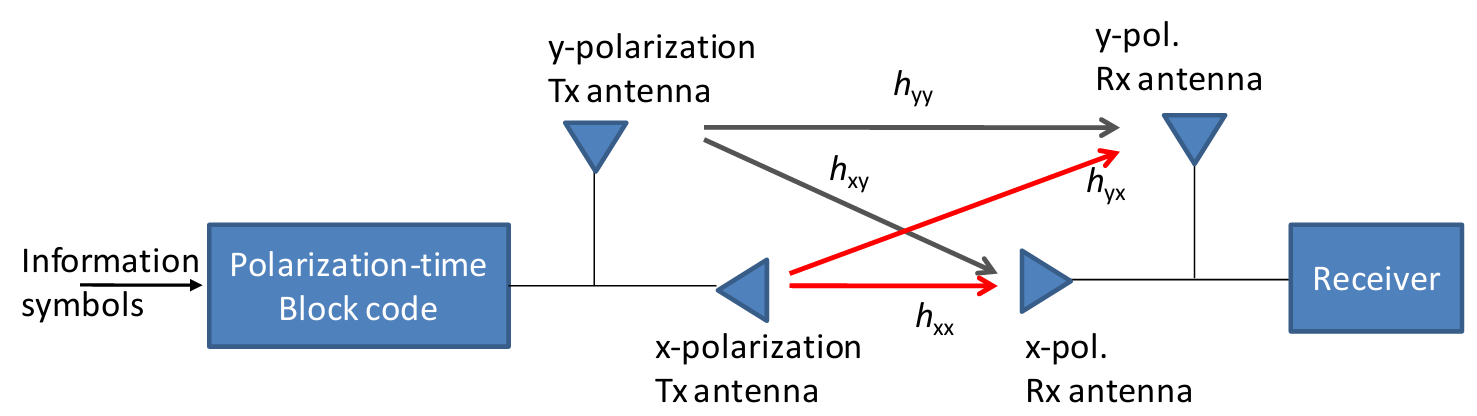
\includegraphics[width=0.8\textwidth]{2x2_polarization_time_coding_mimo.png}}}
			\caption{}
			\label{fig::2x2_polarization_time_coding_mimo}
		\end{figure}

		\item An $(n,k)$ linear block code is described by the following parity-check matrix:
		
		\begin{equationCenter}
			\mathbf{H} = \begin{bmatrix}
				0 & 0 & 0 & 0 & 0 & 0 & 0 & 1 & 1 & 1 & 1 & 1 & 1 & 1 & 1 \\
				0 & 0 & 0 & 1 & 1 & 1 & 1 & 0 & 0 & 0 & 0 & 1 & 1 & 1 & 1 \\
				0 & 1 & 1 & 0 & 0 & 1 & 1 & 0 & 0 & 1 & 1 & 0 & 0 & 1 & 1 \\
				1 & 0 & 1 & 0 & 1 & 0 & 1 & 0 & 1 & 0 & 1 & 0 & 1 & 0 & 1
			\end{bmatrix}
		\end{equationCenter}
		
		\begin{enumerate}
			\item Determine the code parameters of this code: codeword length, number of information bits, code rate, overhead, minimum distance, error correction capability, and error detection capability.

			\item Represent the $\mathbf{H}$-matrix in systematic form and determine the generator matrix $\mathbf{G}$ of the corresponding systematic code. Provide the corresponding shift register based encoding circuit of this systematic code.

			\item The extended code is created by inserting the additional parity-check bits. The most common way of extending the code is by adding an overall parity-check bit. The extended code is then an $(n+1,k)$ code. Determine the bipartite (Tanner) graph of $\mathbf{H}$-matrix of extended code obtained from the original $\mathbf{H}$-matrix above.

			\item Determine the code parameters of the extended code in (c): codeword length, number of information bits, code rate, overhead, minimum distance, error correction capability, and error detection capability.
		\end{enumerate}
		
		\item This problem is related to the \textbf{adaptive modulation and coding applied to 9-ary 2-D constellation} described below, transmitted over wireless channel in the presence of Nakagami fading and AWGN. The eight constellation points in this 2-D constellation are placed on a circle of radius 1. The last (ninth) point is placed in the origin. Assume that the point in the origin appears with probability 0.5, all others with probability 0.5/8. For channel coding use the extended code from Problem 2(c).
		
		\begin{enumerate}
			\item Determine the average symbol error probability for this modulation format in the presence of fading and AWGN.
			
			\item Estimate the coding gain for the extended code from Problem 2(c) and use it in incoming (c)-(e) problems.
			
			\item Determine the optimum power adaptation strategy as well as the corresponding the spectral efficiency of this scheme, in the presence of fading and AWGN.
			
			\item Describe the channel inversion technique for this signal constellation and determine the corresponding spectral efficiency, in the presence of fading and AWGN.
			
			\item Describe the truncated channel inversion technique for this signal constellation and determine the corresponding spectral efficiency, in the presence of fading and AWGN.
		\end{enumerate}
		
		\item In this problem we are concerned with designing an OFDM system that can provide data rate $\geq 50$ Mb/s for available bandwidth of 20 MHz, and which can tolerate the delay spread of up to 100 ns. Provide the design of such a system and describe the corresponding OFDM transceiver.
		
		\item This problem is related to \textbf{coded-modulation applied to 9-ary 2-D constellation} described in Problem 3, in the presence of Nakagami fading and AWGN.
		
		\begin{enumerate}
			\item Describe the transmitter and receiver configuration for 9-ary LDPC-coded modulation for $2 \times 2$ MIMO system.
			
			\item Determine the symbol LLRs required for 3-ary LDPC decoding. Describe how to determine the extrinsic information at the output of 3-ary LDPC decoder for APP demapper. Describe how to determine the prior symbol LLRs for next APP-LDPC decoder iteration step.
		\end{enumerate}
	\end{enumerate}
\end{document}